\documentclass[12pt]{extarticle}
\usepackage{graphicx}
\usepackage{blindtext}
\usepackage{enumitem}
\graphicspath{ {images/} }


\begin{document}

\title{\Huge\textbf{ Technical University Of Varna}}
\author{\huge \textbf{ Can Mert} \\ \\ \Large \textbf{ Faculty no:21625103} \\ \\ \\  \LARGE Socket Programming and Threads} 

\date{}



\maketitle
\newpage
\section{Introduction to Socket Programming}

In the 1980s, the US government's Advanced Research Projects Agency (ARPA) provided
funds to the Universiy of California at Berkeley to implement TCP/IP protocols
under the UNIX operating system. During this project, a group of Berkeley researches
developed an application program interface (API) for TCP/IP network communications
called the socket interface. The socket interface is an API TCP/IP networks it defines
a variety of routines or software functions for the development of applications for TCP/IP networks.
The socket interface designers originally built their interface into the UNIX operating system.
However, other operating systems, environments, such as Microsoft Windows, implement the socket 
interface as software libraries. But it doesnt matter in which of the environment in we program, the code 
will look much the same. Java is preferred language for socket programming but it socket programming can
be done in any language. Java is playform independent, it has exception mechanisms for rebust handling
of common problems that occur during I/O and networking operations and its threading facilities provide
a way to easily implement powerful servers one of java's major strong suits as a programming language for
client-server application development is its wide range of network support. Java has this advantage 
because it was developed with the Internet in mind. Another advantage of java is that it provides 
security. The result is that we have a lot of options in regard to network programming in Java.
Java performs all of its network communication through sockets.

\subsection{Client-Server Communcation}

A network is composed  of computers which is either a client or server. A server is a program that
is offering some services whereas a client is a program that is requesting some service, Servers are powerful
computers or processes dedicated to managing disk drives (file servers), printers (print servers), or
network traffic (network services) whereas clients are PCs or workstations on which users run applications.
Clients need servers for resources, such as files, devices and even processing power. When these programs are 
executed, as a result, a client and a server process are created simultaneously and this two processes 
communicate with each other by reading from and writing to sockets.

\begin{center}

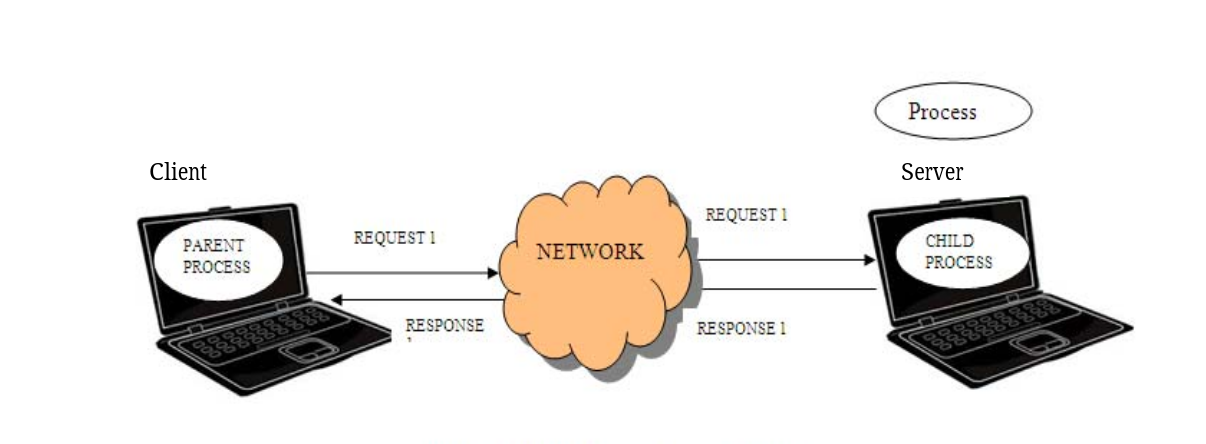
\includegraphics[width=15cm, height=11cm]{client-server communication}

    1.1 Client-Server communications

\end{center}

These sockets are the programming interfaces provided by the UDP and TCP protocols
for stream and datagram communication respectively of the transport layer which is
a part of the TCP/IP stack. When creating a network application, the developer's 
main task is to wride code that for the both client and server programs, and the 
developer needs to complete control over what goes in the code. Code does not implement
a public-domain protocol, so other independent developers will not be able to develop code
that interoperates with the application. When developing a proprietary application,
developer should be careful not to use one of the well-known port numbers defined in RFCs.

\subsection{Sockets}

The term that 'socket' comes from an electricity/phone socket metaphor where sockets 
acts as interfaces that plug into each other over a network. \\
Technically, sockets are defined in many ways; \\

\begin{enumerate}[label=\textbf{\arabic*}]
    
\item According to Wikipedia, a network socket is an endpoint of an inter-process
communcation flow across a computer network. A socket is composed of an IP  address
and a port number.

\item Sockets can be defined as the end-points of a connection between two computers identified
by an IP Address and a port number.

\item Also sockets can also be defined as a software abstraction used to represent the "terminals" of a
connection between two machines.

\item Socket is the door between the application process and TCP.

\item Socket is an interface between the application and the network.

\item Socket also can be defined as an abstraction that is provided to an application programmer to send or 
receive data to another process.

\end{enumerate}

\subsection{Operations of Socket}

A socket performs four main operations:

\begin{enumerate}[label=\textbf{\arabic*}]

\item To connect to a remote machine
\item Send data
\item Receive data
\item Close the connection

\end{enumerate}

A socket may not be connected to more than one host at a time. However, a socket may both send data
to and receive data from the host to which its connected. The java.net.Socket class is Java's interface
to a network socket and its allows you to perform all four fundamental socket operations.

\subsection{Port}

In computer networking, a port is an applicatiton-specific or process-specific software construct
serving as a communications endpoint in a computer's host operating system. A port is associated with an
IP address of the host, as well as the type of protocol used for communication.
The purpose of ports is to uniquely identify different applications or processes running on a single computer.
The protocols that primarily use ports are the Transport Layer protocols, such as the Transmission
Control Protocol (TCP) and the User Datagram Protocol (UDP) of the Internet software stack, often
called TCP/IP (Transport Control Protocol/Internet Protocol) stack, as shown in that figure:1.4.
They use ports to map incoming data to a particular process running on a computer. So a port will
identify a socket on a host.


\begin{center}

    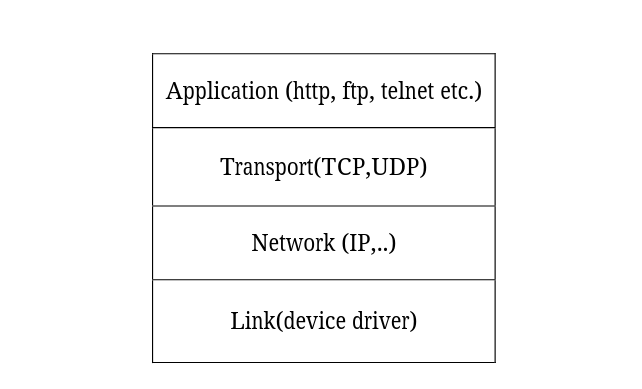
\includegraphics[width=15cm, height=11cm]{TCP-IP software stack}
    
        1.4 TCP/IP software stack
    
 \end{center}

 Still, an IP address is not enough to identify a unique server, because many server programs may
 exist on one machine. So we need a unique identification for each server. This unique identification
 called as port. \\ \\

 When we are setting up client or a server we must choose a port to where both client and server are
gonna meet. This port not a physical port, but a logical port specified by a 16-bit integer number.
But some port numbers from 0 to 1024 has been reserved to support common/well known services.
And we need to be careful not to use one of that port numbers defined in the RFCs while developoing a
proprietary client-server application.

\begin{itemize}

    \item ftp 21/tcp
    \item telnet 23/tcp
    \item smtp 25/tcp
    \item login 513/tcp
    \item http 80/tcp,udp
    \item https 443/tcp,udp
    
\end{itemize}

User-level process/services generally use port number value >= 1024

\section{Network Programming With Sockets}

The Internet has been very popular in the past few years. While its still growing this also 
increased demand for Internet network software as well. One of the biggest advantages to developing
Internet software with Java is in its robust networking support built into the core language.
The java.net package provides us with classes that representing URLs, URL connections and sockets.
Combined with java.io package, we can quite easily write sophisticated platform-independent applications.
Network programming makes use of socket for Interprocess Communication. BSD socket interface supports
different domain, the UNIX domain, the Internet Domain and the NS Domain. Java simply supports the
Internet domain to maintain cross platform. In Internet domain, the BSD Socket Interface is built
on the top of either TCP/IP or UDP/IP or the raw Socket. Socket programming is important to undderstand
how internet based communication work but not at the level program developed but at a higher
level that is compiled to set of Socket Programs.

\subsection{Socket Programming With TCP}

TCP provides a connection oriented service, since it is based on connections between clients
and servers. This means that a connection is established before processes can exchange data. The
Transmission Control Protocol is also reliable because when a TCP client sends data to the server,
it requires an acknowledgement in return. If its not received, then TCP automatically retransmit
the data and waits for a longer period of time. The processes running on different machines communicate
with each other by sending messages into sockets. Each process is similar to a house and the process's 
socket is analogous to a door. As you can see in figure 2.1, the socket is the door between the application
process and TCP.

\begin{center}

    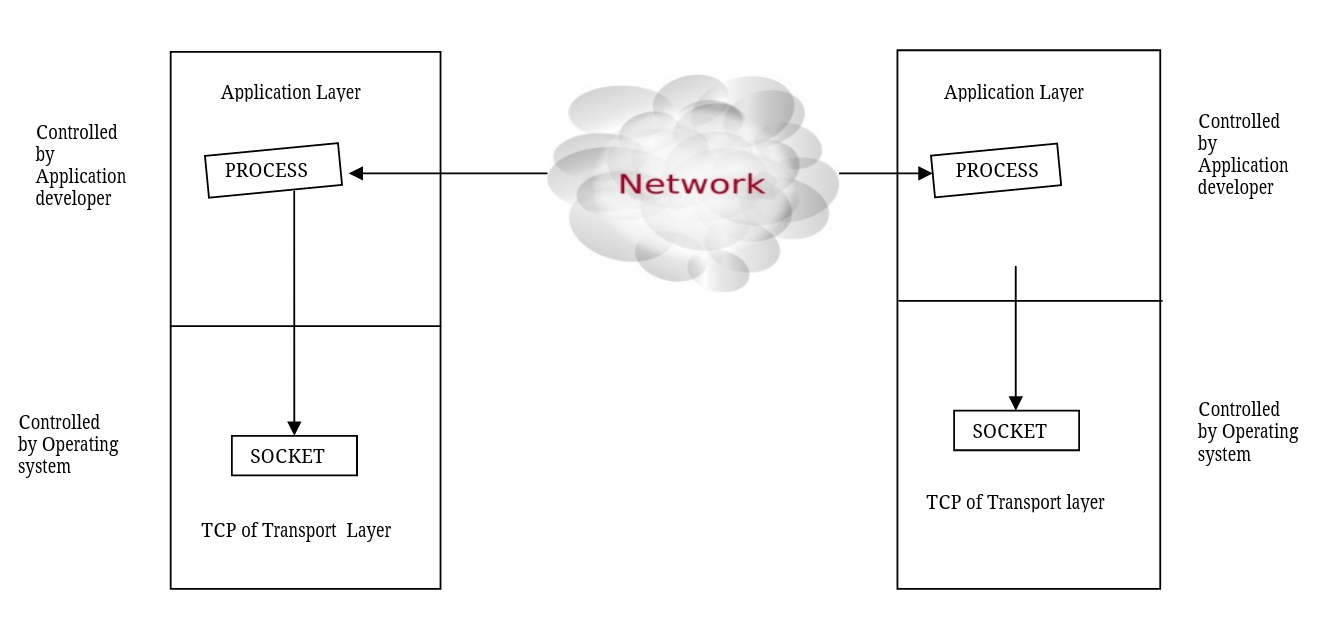
\includegraphics[width=15cm, height=9cm]{Process through TCP sockets}
    
        2.1 Process communicating through TCP sockets
    
\end{center}

The application developer has control of everything on application-layer side of the sicket. However
it has little control of the transport-layer side. TCP guarantees thatt the server process will receive
each byte in the order sent. Furthermore, the client process can also receive bytes from its socket
and the server process can also send bytes into its connection socket. This happens in Figure 2.2.

\begin{center}

    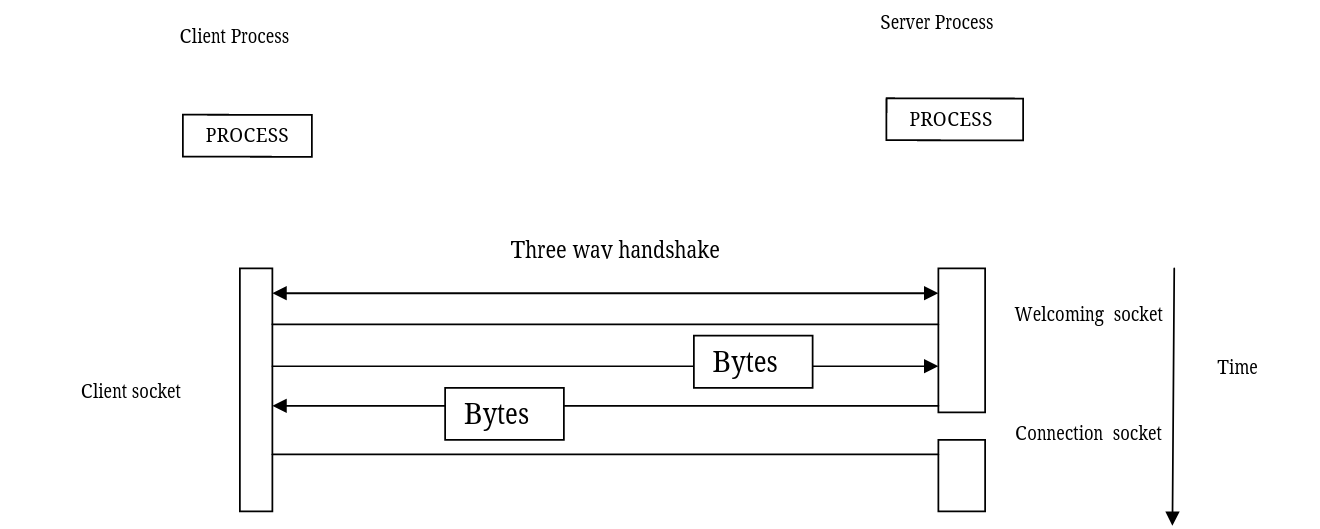
\includegraphics[width=15cm, height=12cm]{client-welcoming-connection socket}
    
        2.2 Client socket, welcoming socket, and connection socket
    
\end{center}

Because sockets play a central role in client/server applications, client/server application is also
called to as socket programming.

\subsection{Socket programming over TCP in Java}

Java has provided the facility to create sockets for interprocess communication (IPC). So while 
programming for sockets in java, we have to make sure to import the java.net.package. This package 
provides a class so that socket implement the client side connection. And a class ServerSocket implements
the server side connection. The Server Socket on the server performs the methods "bind" which is to fix
to a certain port no. and IP address, "listen" to wait for incoming requests on the port and "accept"
for acceptance of connection from the client respectively. Upon acceptance, the server gets a 
new socket bound to the same local port and also has its remote endpoint 
set to the name of the  machine  and  port  of  the  client.  So the client  
initiates a three way handshake with the server and creates a TCP connection  
with the server. So now client and server can communicate by writing or reading from their sockets.
And when its done, the close method is called from both client and the server for closing the connection
as shown in this figure 2.3 below.

\begin{center}

    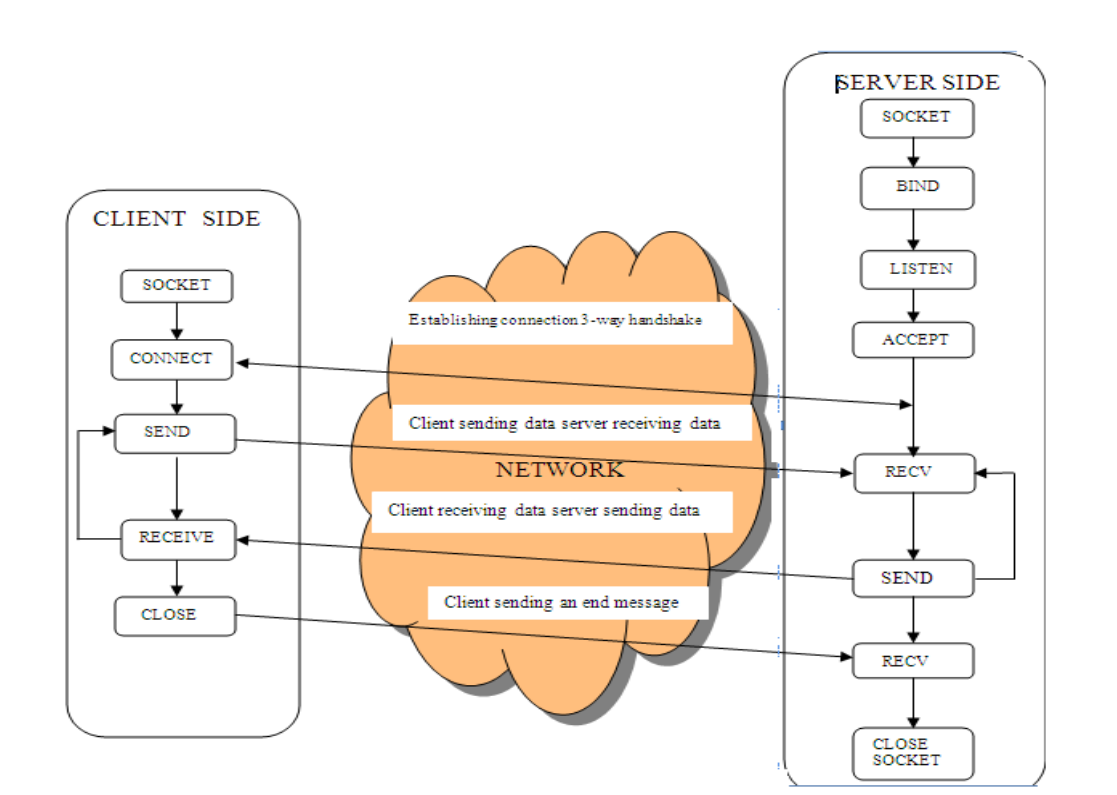
\includegraphics[width=15cm, height=9cm]{TCP client-server}
    
        2.3 TCP client-server
    
\end{center}

List of methods provided by the Berkeley sockets API library:

\begin{itemize}

    \item socket() creates a new socket of a type, identified by an integer number and allocates resources to it.
    \item bind() is associates a socket with a socket address structure, a specified local port number and IP address. Its typically used on the server side.
    \item listen() is used on the server side, and causes a bound TCP socket to enter listening state.
    \item connect() is used on the client side, and assigns free local port number to a socket. For the TCP socket it attempts to establish a new TCP connection.
    \item accept() is used on the server side. This accepts a received incoming attempt to create a new TCP connection from remote client, and creates a new socket with the address pair of this connection.
    \item send(),recv(),write(),read(),sendto() and recvfrom() used for sending and receiving data to/from a remote socket.
    \item close() makes the system to release resources allocated to a socket. For the TCP, the connection is terminated.

\end{itemize}

\subsection{Socket Programming over UDP}

UDP is a connection-less, datagram protocol. The client doesnt establish connection with the server like in case of TCP.
Instead, the client just sends a datagram to the server using the sendto function and this requires
address of the destination as a parameter. Similarly, the server does not accept a connection from a client.
Instead, the server just calls the recvfrom function, which waits until data arrives from some client.
Recvfrom returns the IP address of the client, along with the datagram, so the server can send a response to the client
as shown in figure below 2.4.

\begin{center}

    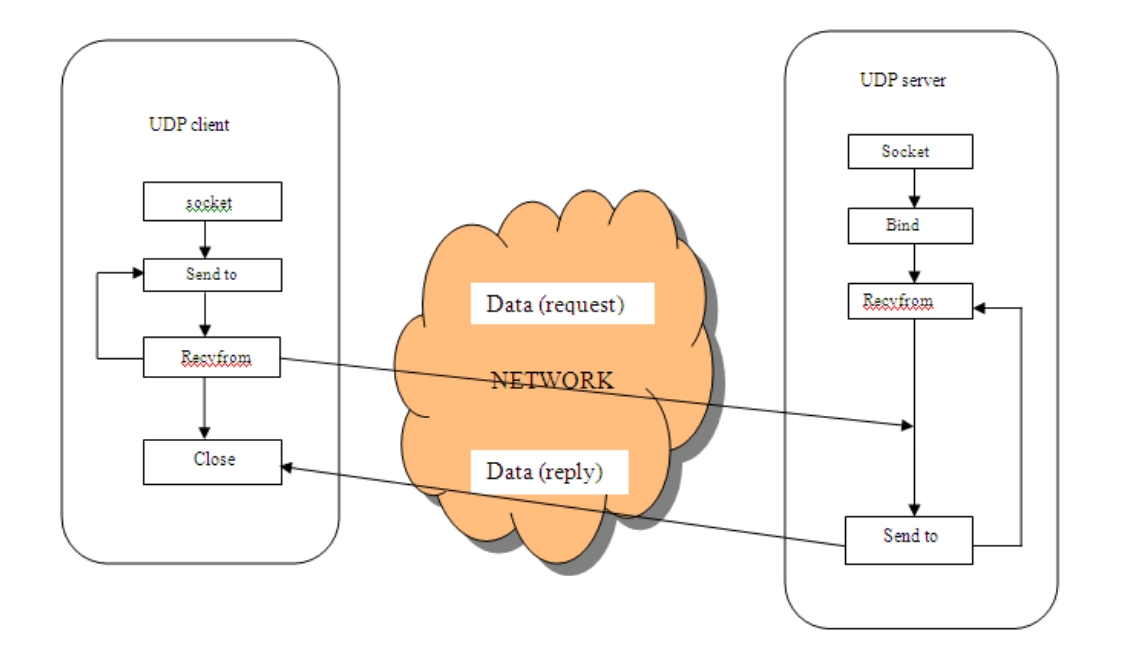
\includegraphics[width=15cm, height=5cm]{UDP client-server}
    
        2.4 UDP client-server
    
\end{center}

There is no any initial handshaking. When you send a data or message, you dont know if it will
get there, it could get lost on the way so it lacks reliability. There also may be corruption
while transferring a message.
UDP Socket's list of functions down below:

\begin{itemize}
    \item socket() both client and the server creates the function.
    \item bind() its usually used on the server side and bounds socket with a socket address structure, specified local port.
    \item listen() This typically used on the server side waiting for incoming connections from client as passive.
    \item sendto() It is on both sides used to send a datagram to another UDP socket.
    \item recvfrom() It is on both client side and server side. It is used to receive a datagram from another UDP socket.
    \item close() closes a socket.
\end{itemize}

\section{References}

\begin{itemize}

    \item http://en.wikipedia.org/wiki/Berkeley Sockets.
    \item Joseph M. Dibella ,  “Socket Programming with Java"
    \item http://www.tutorialspoint.com/java/javanetworking.htm
    
\end{itemize}

\newpage

\section{Threads}

A thread is a basic unit of CPU utilization, consisting of a program counter, a stack, and a set of registers,(and a thread ID).
Traditional(heavyweight) processess have a single thread of control-There is one program counter, and one sequence of instructions that can
be carried out at any given time. If you look at the figure below, multi-threaded appliciations have multiple
threads within single process, each having their own program counter, stack and set of registers, but sharing
common code,data, and certain structures like open files.


\begin{center}

    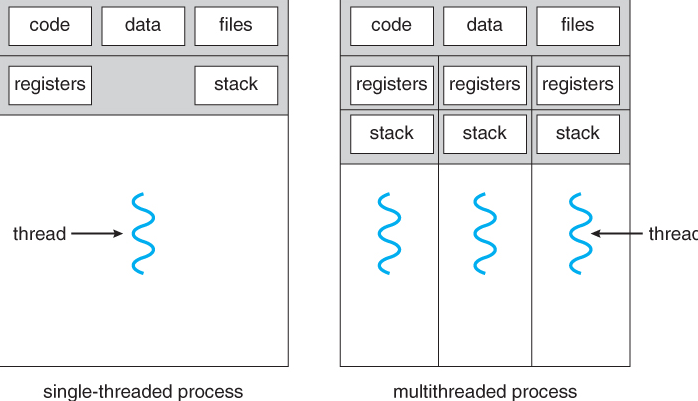
\includegraphics[width=15cm, height=12cm]{thread}
     
\end{center} 

\newpage

\subsection{Why Threads?}

\begin{itemize}

    \item Threads are very useful in modern programming whenever a process has multiple tasks to perform independently of the others.
    \item This is particularly true when one of the tasks may block, and it is desired to allow the other tasks to proceed without blocking.
    \item For example in a word processor, a background thread may check spelling and grammar while a foreground thread processes user input ( keystrokes ), while yet a third thread loads images from the hard drive, and a fourth does periodic automatic backups of the file being edited.
    \item Another example is a web server - Multiple threads allow for multiple requests to be satisfied simultaneously, without having to service requests sequentially or to fork off separate processes for every incoming request. ( The latter is how this sort of thing was done before the concept of threads was developed. A daemon would listen at a port, fork off a child for every incoming request to be processed, and then go back to listening to the port. )
    
\end{itemize}

\begin{center}

    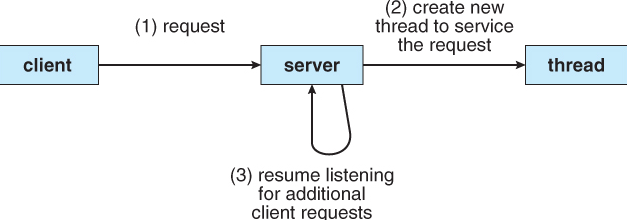
\includegraphics[width=15cm, height=9cm]{multithreaded}
     
\end{center} 

\subsection{Benefits}

There are four main categories of benefits to multi-threading

\begin{itemize}
    \item Responsiveness - One thread may provide rapid response while other threads are blocked or slowed down doing intensive calculations.
    \item Resource Sharing - By default threads share common code, data, and other resources, which allows multiple tasks to be performed simultaneously in a single address space.
    \item Economy - Creating and managing threads is much faster than performing the same tasks for processes.
    \item Scalability and Utilization of multiprocessor architectures - A single threaded process can only run on one CPU, no matter how many may be available, whereas the execution of a multi-threaded application may be split amongst available processors.
\end{itemize}

\subsection{Thread States}

Primary States:
\begin{itemize}
    \item Running, Ready and Blocked.
\end{itemize}

Operations to change state:
\begin{itemize}
    \item Spawn: new thread provided register context and stack pointer.
    \item Block: event wait, save user registers, PC and stack pointer.
    \item Unblock: moved to ready state.
    \item Finish: deallocate context and stacks.
\end{itemize}

\newpage 

\section{User and Kernel Level Threads}

\subsection{Kernel-Level Threads}

To make concurrency cheaper, the execution aspect of process is separated out into threads. As such, the OS now manages threads and processes. All thread operations are implemented in the kernel and the OS schedules all threads in the system. OS managed threads are called kernel-level threads or light weight processes.
In this method, kernel knows about and manages  the threads. No runtime system is needed. OS kernel provides system call to 
create and manage threads. \\ 

Advantages:

\begin{itemize}
    \item Because kernel has full knowledge of all threads, Scheduler may decide to give more time to a process having large number of threads than process having small number of threads. 
    \item Kernel-level threads are especially good for applications that frequently block. \\ \\
    Disadvantages:
    \item The kernel-level threads are slow and inefficient. For instance, threads operations are hundreds of times slower than that of user-level threads. 
    \item Since kernel must manage and schedule threads as well as processes. It require a full thread control block (TCB) for each thread to maintain information about threads. As a result there is significant overhead and increased in kernel complexity. 
\end{itemize}

\subsection{User-Level Threads}

Kernel-Level threads make concurrency much cheaper than process because, much less state to allocate and initialize. However, for fine-grained concurrency, kernel-level threads still suffer from too much overhead. Thread operations still require system calls. Ideally, we require thread operations to be as fast as a procedure call. Kernel-Level threads have to be general to support the needs of all programmers, languages, runtimes, etc. For such fine grained concurrency we need still "cheaper" threads.

Advantages:

\begin{itemize}
    \item The most obvious advantage of this technique is that a user-level threads package can be implemented on an Operating System that does not support threads. 
    \item Simple Representation: Each thread is represented simply by a PC, registers, stack and a small control block, all stored in the user process address space. 
    \item Simple Management:  This simply means that creating a thread, switching between threads and synchronization between threads can all be done without intervention of the kernel. 
    \item Fast and Efficient:  Thread switching is not much more expensive than a procedure call.  \\ \\
    Disadvantages:
    \item User-Level threads are not a perfect solution as with everything else, they are a trade off. Since, User-Level threads are invisible to the OS they are not well integrated with the OS.
\end{itemize}


\section{Multithreading Models}

\begin{itemize}
    \item There are two types of threads to be managed in a modern system:User threads and kernal threads.
    \item User threads are supported above the kernel, without kernel support. These are the threads that application programmer would put into their programs.
    \item Kernel threads are supported within the kernel of the OS itself. All modern OSes support kernel level threads, allowing the kernel to perform multiple simultaneous taks and/or to service multiple kernel system calls simultaneously.
    \item In a specific implementation, the user threads must be mapped to kernel threads, using one of the following strategies.
\end{itemize}

\subsection{Many-To-One Model}

\begin{itemize}
    \item In this model many user-level threads all mapped to onto a single kernel thread.
    \item Thread library handled thread management in the user space, which is very efficient.
    \item But if a blocking system call is made, then entire process blocks, even if the other user threads would otherwise be able to continue.
    \item Because a single kernel thread can operate only on a single CPU, the many-to-one model does not allow individual processes to be split across multiple CPUs.
    \item Few systems uses this model like Solaris Green Threads, Gnu Portable Threads
\end{itemize}

\begin{center}

    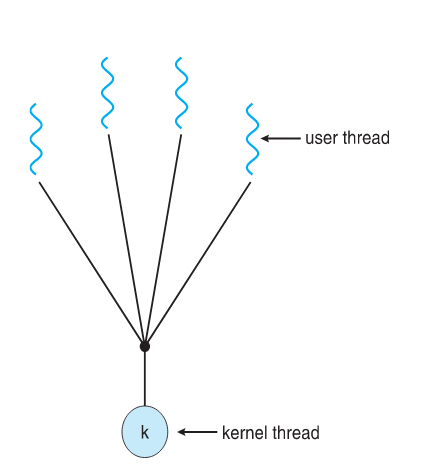
\includegraphics[width=15cm, height=10cm]{many-to-one}
     
\end{center} 

\subsection{One-To-One Model}

\begin{itemize}
    \item Each user-level thread maps to kernel thread.
    \item Creating a user-level thread creates a kernel thread.
    \item More concurrency than many-to-one.
    \item Number of threads per process sometimes restricted due to overhead.
    \item Examples; Windows,Linux,Solaris 9 and later.
\end{itemize}

\begin{center}

    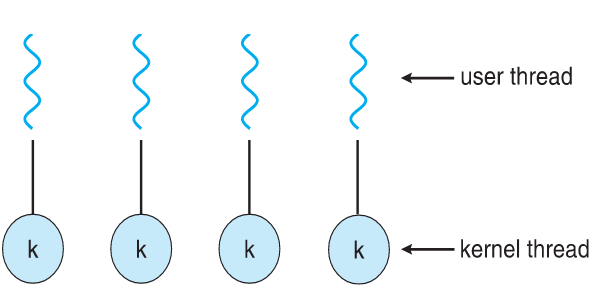
\includegraphics[width=15cm, height=8cm]{one-to-one}
     
\end{center} 

\newpage

\subsection{Many-To-Many Model}

\begin{itemize}
    \item Allows many user to level threads to be mapped to many kernel threads.
    \item Allows the operating system to create a sufficient number of kernel threads.
    \item Solaris prior to version 9
    \item Windows with the ThreadFiber package.
\end{itemize}

\begin{center}

    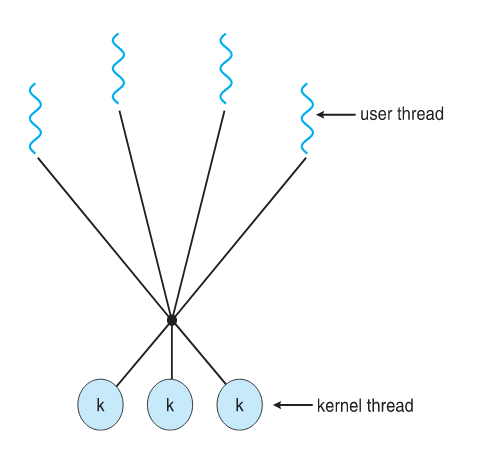
\includegraphics[width=15cm, height=8cm]{many-to-many}
     
\end{center} 

\newpage

\subsection{Two-Level-Model}

\begin{itemize}
    \item Similar to M:M, except that it allows a user thread to be bound to kernel thread.
    \item Examples: IRIX, HP-UX, Tru64 UNIX, Solaris 8 and earlier.
\end{itemize}

\begin{center}

    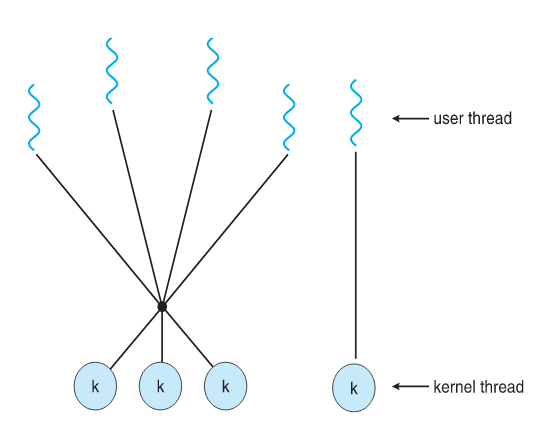
\includegraphics[width=15cm, height=8cm]{two-level}
     
\end{center} 

\section{References}
\begin{itemize}
    \item Abraham Silberschatz, Greg Gagne, and Peter Baer Galvin, "Operating System Concepts, Ninth Edition ", Chapter 4 
    \item https://www.geeksforgeeks.org/threads-and-its-types-in-operating-system/
\end{itemize}






















\end{document}

